\section{Data Visualization}
\label{sec:datavis}

% extracting information out of data

The aim of data visualization is to make large datasets understandable.
Visualizating data transforms it into information. Data itself is just noise, whereas information holds value. In what way data needs to be transformed is determined by context [\cite{terganKnowledgeInformationVisualization2005}].

Aside from design fundamentals, most specialized resources discuss visualization types intended for interrelated data. Interpreting such complex information requires time and cognitive capacity unavailable in scenarios such as those mentioned in Section \ref{sec:CPC}. In these situations, a clear picture of the current status must be available at all times, which only allows for individual data values and therefore limits the number of possible visualization types.

Ferdio, an agency specialized on infographics and data visualization, has created a library of visualization types\footnote{\href{https://datavizproject.com/}{Data Viz Project | Collection of data visualizations to get inspired and find the right type}}. In this library, out of a 166 options, nine are for single data.

\begin{figure}[hbt]
    \centering
    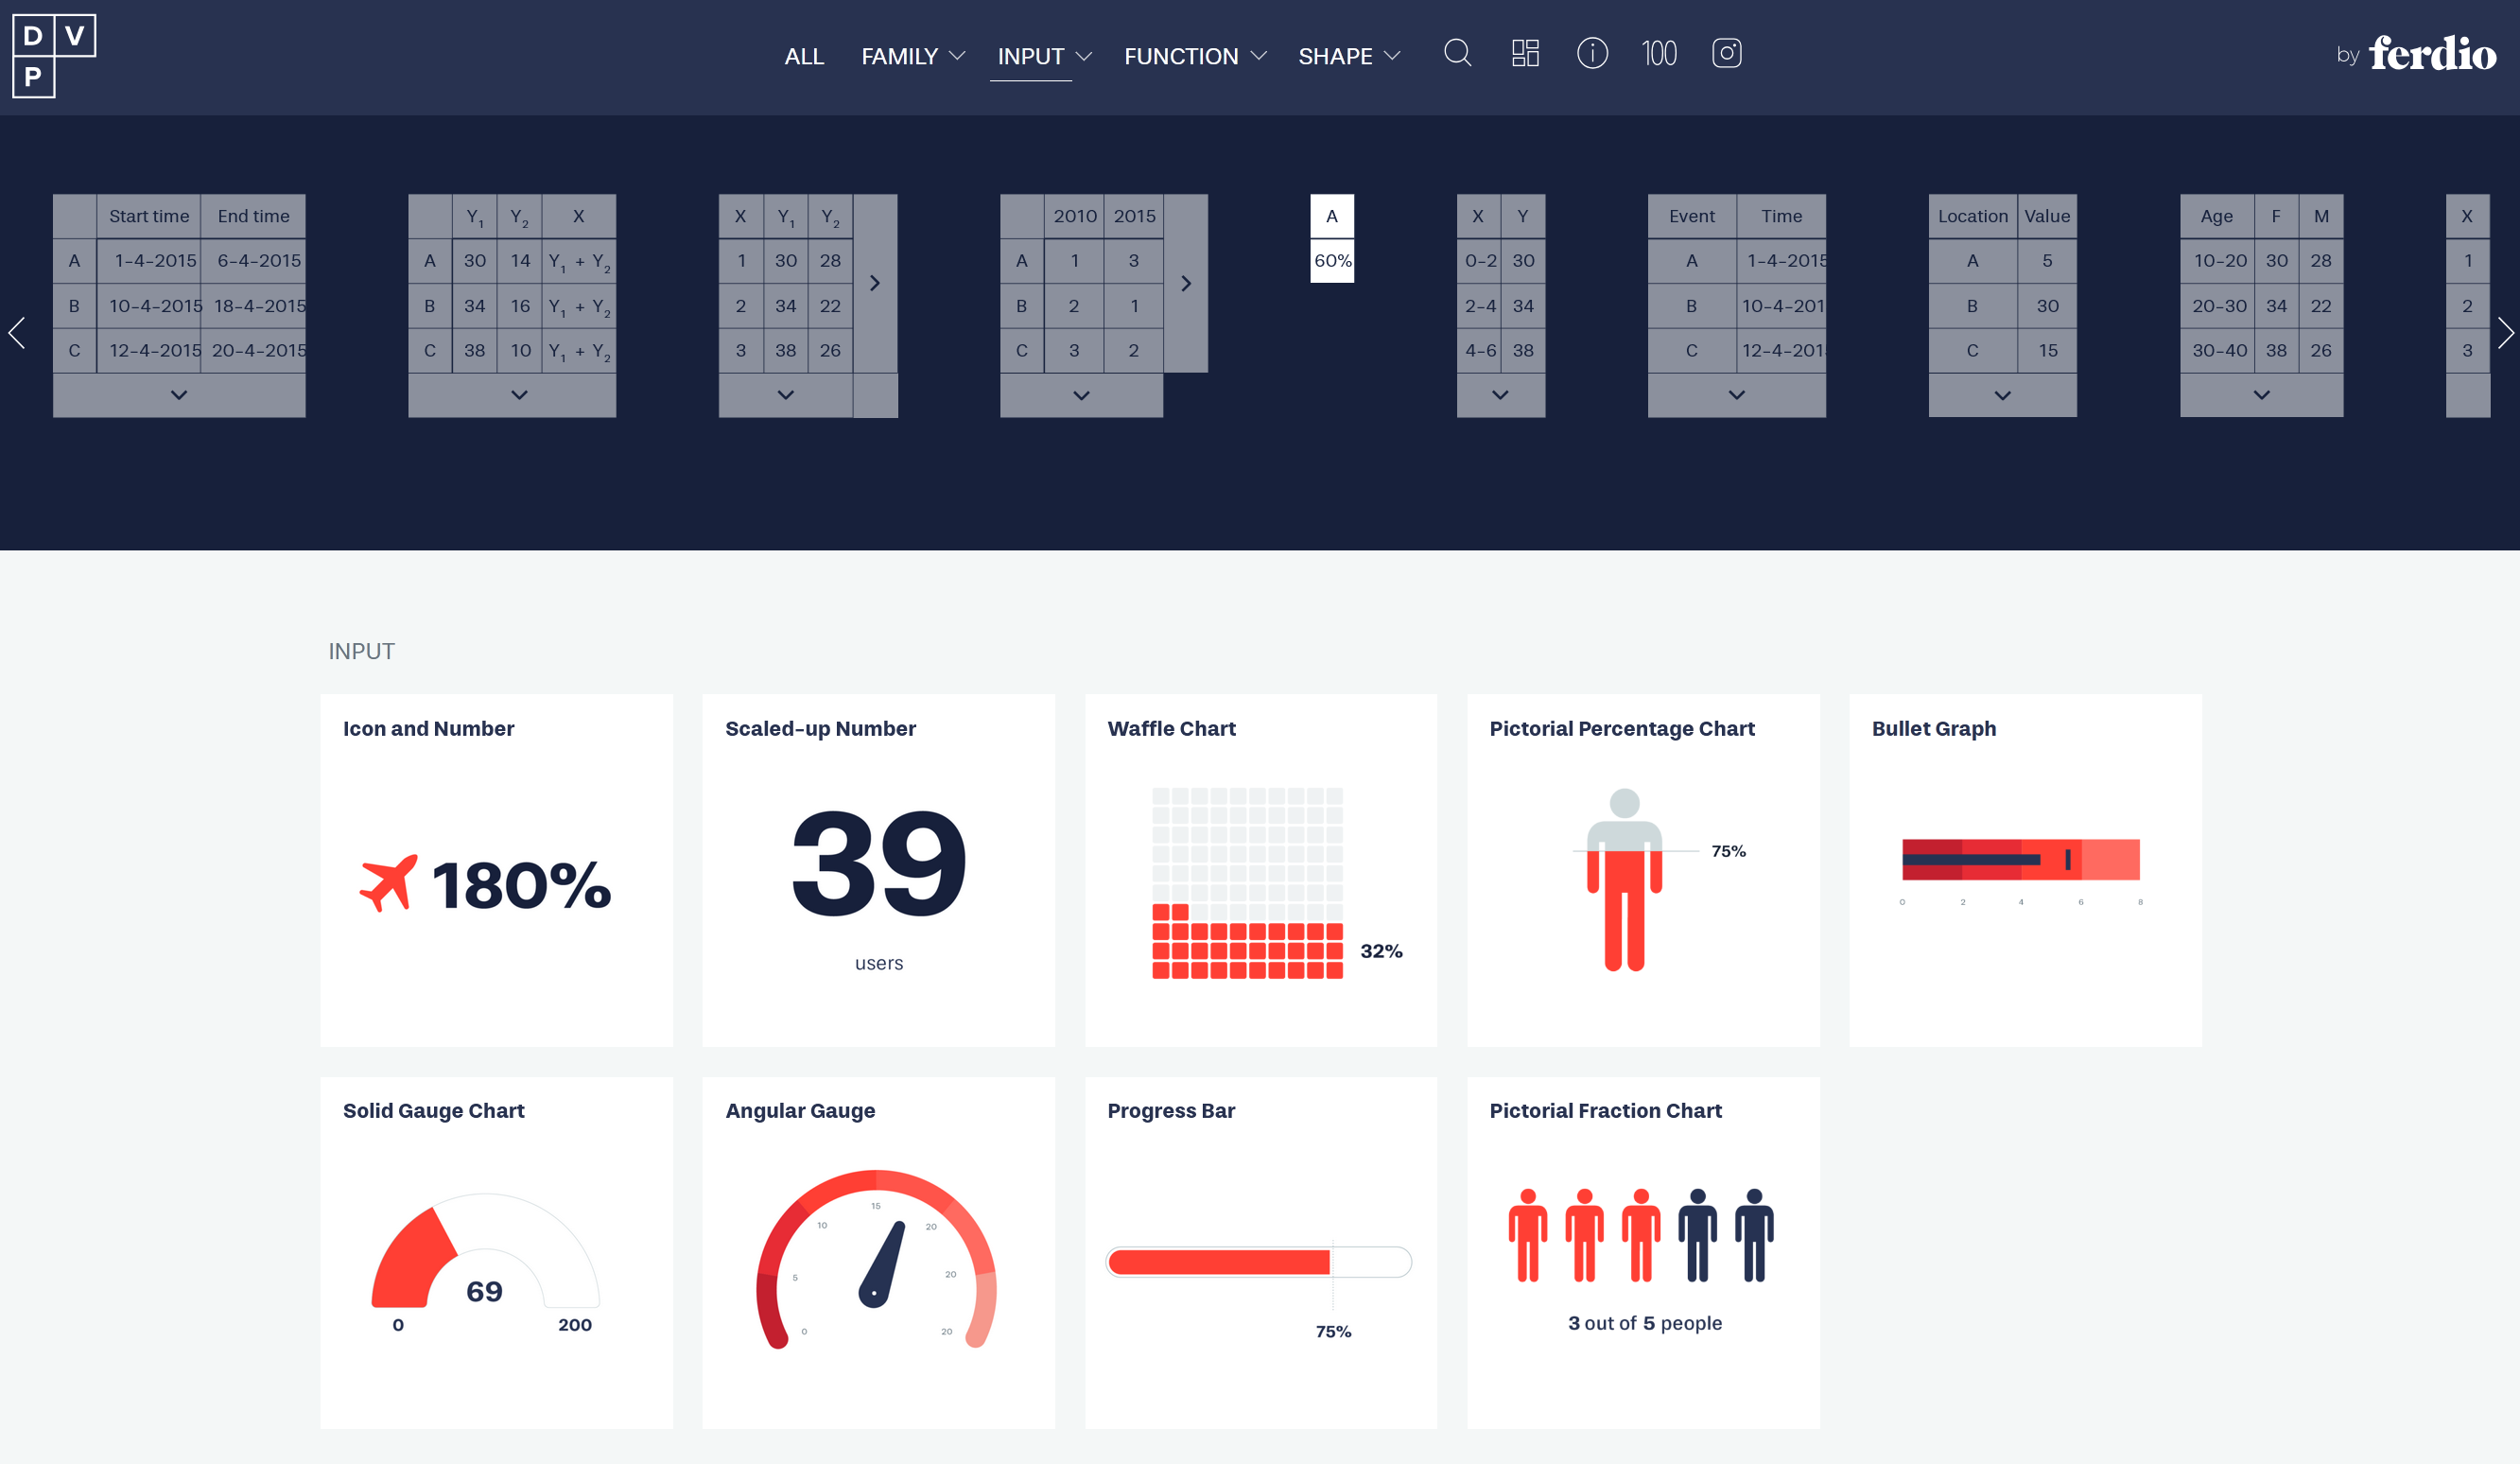
\includegraphics[width=1\textwidth]{assets/ferdio_single_data_page.png}
    \caption{The options for single data (highlighted in the menu bar) in Ferdio's data visualization library.}
    \label{fig:ferdio_single_data}
\end{figure}

%Visual variables correspond to the fundamental design elements
\textcite{wilke2VisualizingData2019} lists position, shape, size and color as basic elements for visualization. Position describes the placement of data, related to other points or axes of a diagram. For color, hue and value should be distinguished, since they are suited for different kinds of data. Hues tend to work better for distinctive categories. Value for continuous data GRADIENTS, the eye is much more sensitive to differences in lightness (see Section \ref{sec:HVS_attention}).
Hues can also be used for gradients (e.g. rainbow), but require much more intention to work.

% Purposes of color to convey information are grouping or relationships. Grouping is necessary for the HUD, but is managed by the spatial location of and the spacing between elements.
% visual encoding of information: encoding works by highlighting differences (e.g. if a monochrome display is green, the color green holds no meaning)

Each of these elements can be used to encode information. Which element is used for which information influences the type of visualization. Importantly, this mapping must be unique, else it becomes ambiguous and obscures the meaning [\cite{wilke2VisualizingData2019}].

% \cite{behrischQualityMetricsInformation2018}
% - fig 3: metrics categorized by cognitive complexity
% - component design focuses on mid-level perception and relating design patterns (reducing clutter, task effectiveness, details on demand)
% - planned notification system exploits low-level perception (preattentive processing, gestalt laws, change blindness)
% - visual patterns to intuitively understand mathematical patterns
% - signal-to-noise ratio

\subsection*{Visualizations for Single Value Data}

\textbf{Icons and Scaled-up Numbers.}
highlight a single value
Often used when the number does not need a context or a comparison
icons serve as description or label

\textbf{Differential Indicators.}

These are a type of status indicator, and meant to visualize changes of information. arrows
stock values, red green

\textbf{Solid and Angular Gauges.}
solid necessarily show specific data/numbers, more for abstract status evaluation
Angular Gauge uses a radial scale for specific data points (e.g. temperature)
dial over a radial scale with defined limits

According to \textcite{xiaVisualizingWristImpact2025}, bar charts outperform radial visualization.

\textbf{Status Bar.}
A progress bar is a graphical control element used to visualize the progression of an extended operation, such as a download, file transfer, or installation. Sometimes, the graphic is accompanied by a textual representation of the progress in a percent or quantitative format.
